%% LyX 2.2.2 created this file.  For more info, see http://www.lyx.org/.
%% Do not edit unless you really know what you are doing.
\documentclass[12pt]{article}
\usepackage[T1]{fontenc}
\usepackage[latin9]{inputenc}
\usepackage[letterpaper]{geometry}
\geometry{verbose,tmargin=1.25in,bmargin=1.15in,lmargin=1in,rmargin=1in}
\usepackage{fancyhdr}
\pagestyle{fancy}
\usepackage{xcolor}
\usepackage{refstyle}
\usepackage{float}
\usepackage{calc}
\usepackage{amsmath}
\usepackage{graphicx}
\usepackage{setspace}
\PassOptionsToPackage{normalem}{ulem}
\usepackage{ulem}
\onehalfspacing
\usepackage[unicode=true,pdfusetitle,
 bookmarks=true,bookmarksnumbered=false,bookmarksopen=false,
 breaklinks=true,pdfborder={0 0 0},pdfborderstyle={},backref=false,colorlinks=false]
 {hyperref}

\makeatletter

%%%%%%%%%%%%%%%%%%%%%%%%%%%%%% LyX specific LaTeX commands.

\AtBeginDocument{\providecommand\eqref[1]{\ref{eq:#1}}}
%% Because html converters don't know tabularnewline
\providecommand{\tabularnewline}{\\}
\RS@ifundefined{subsecref}
  {\newref{subsec}{name = \RSsectxt}}
  {}
\RS@ifundefined{thmref}
  {\def\RSthmtxt{theorem~}\newref{thm}{name = \RSthmtxt}}
  {}
\RS@ifundefined{lemref}
  {\def\RSlemtxt{lemma~}\newref{lem}{name = \RSlemtxt}}
  {}


%%%%%%%%%%%%%%%%%%%%%%%%%%%%%% User specified LaTeX commands.
\usepackage{lipsum}

%\pagestyle{fancy}  
\fancyhead{} % clear all header fields  
\fancyfoot{} % clear all footer fields 
\renewcommand{\headrulewidth}{0pt} % no line in header area  
\renewcommand{\footrulewidth}{0pt} % no line in header area

\cfoot{\thepage}
\makeatletter
\let\ps@plain\ps@fancy   % Plain page style = fancy page style
\makeatother

\usepackage{listings}
\lstset{
basicstyle=\small\ttfamily,
columns=flexible,
breaklines=true
}

\usepackage{helvet} % add in some fonts

% rename table of contents
%\usepackage[norsk]{babel}
%\addto\captionsnorsk{%
%\renewcommand{\contentsname}{Table of Contents}}

\AtBeginDocument{\renewcommand\contentsname{Table of Contents}}

\usepackage{subcaption}
\usepackage{cleveref}

\newcommand\numberthis{\addtocounter{equation}{1}\tag{\theequation}}

\makeatother

\begin{document}
\begin{figure}[t]
\vspace*{0.5in}

\centering{}
\includegraphics[width=1.25in]{afrl}
\end{figure}


\title{\textbf{TGF Transonic Validation Report}}
\maketitle
\begin{singlespace}
\begin{center}
{\small{}prepared by}
\par\end{center}{\small \par}
\end{singlespace}

\begin{center}
\textbf{Lt Dayle Chang AFRL/RQVX} 
\par\end{center}

\begin{center}
in coordination with
\par\end{center}

\begin{center}
\textbf{Dr. Aaron Altman AFRL/RQVX}\\
\textbf{Bob Guyton AFRL/RQVX}
\par\end{center}

\vfill{}

\noindent{\fboxrule 0.6pt\fboxsep 8pt\fcolorbox{black}{lightgray}{\begin{minipage}[t]{1\columnwidth - 2\fboxsep - 2\fboxrule}%
{\small{}\uline{DISTRIBUTION STATEMENT C}}{\small{} - Distribution
authorized to U.S. Government agencies and their contractors; Critical
Technology; 15 Mar 2017. Other requests for this document shall be
referred to AFRL/RQVX}%
\end{minipage}}}

\vspace*{\bigskipamount}


\cfoot{\textbf{{\fontfamily{ptm}\selectfont FOR OFFICIAL USE ONLY}}}

\pagebreak{}

\chead{\textsf{\textbf{\small{}{\fontfamily{phv}\selectfont \small UNCLASSIFIED // FOR OFFICIAL USE ONLY}}}}

\cfoot{\thepage}

\begin{singlespace}
\tableofcontents{}

\vspace*{0.75in}

\listoffigures

\vspace*{0.75in}

\listoftables

\end{singlespace}

\pagebreak{}

\section{Introduction}

\pagebreak{}

\section{Analysis}

We started re-running the data and I started noticing that the pre-run
windoff data was different than the post-run windoff data. The pre-
and post- run windoff data for the 2 days of testing are shown in
fig 1 and 2. We wanted to see if this was just an effect of tube lag
so we sampled the wind-off once more about 1 or 2 minutes later and
then sampled some more after the model change (fig 3). The results
led me to believe that there's a lot more lag than we thought and
that the lag was greatest at windoff, since the pressure differential
is lowest. To see if this was true, we went on condition and waited
5 minutes before acquiring data and compared it to the same runs from
before (fig 4-6: higher pressure profiles are the ones acquired after
5 min.) and saw some differences. If this really is due to tube lag,
we should be able to see the pressure profiles change from the one
profile to the other profile if we sampled the data over a longer
period of time. On a side note, the 'ATMOS' tag in the plot title
refers to plots that have the standard atmosphere correction we talked
about applied. We did a time sample study for about 10 minutes collecting
data every minute and in figures 7-9 you can see the profile \textquotedbl{}change\textquotedbl{}
from one to the other. The delta pressure between profiles show that
our standard atmosphere correction isn't quite perfect, but gets us
close. Finally, the static and total streamwise pressure profiles
are plotted in figures 10 through 12 with the extra station 3 profile
reflecting data acquired after 10 minutes of going on condition.

Streamwise Normalized Plots. The static and totals see a much smaller
percent difference (because they're absolute) and the dynamics see
a much larger percent difference (2-15\% difference). 

\begin{figure}[p]
\centering{}\includegraphics[width=3in]{\string"more_plots/1 Pre- and Post- WindOff Comparisons on 14-Aug STATIC\string".png}\caption{some caption}
\end{figure}

\begin{figure}[p]
\centering{}\includegraphics[width=3in]{\string"more_plots/2 Pre- and Post- WindOff Comparisons on 15-Aug STATIC\string".png}\caption{}
\end{figure}

\begin{figure}[p]
\centering{}\includegraphics[width=3in]{\string"more_plots/3 Post-Windoff Recovery on 15-Aug STATIC\string".png}\caption{}
\end{figure}

\begin{figure}[p]
\centering{}\includegraphics[width=3in]{\string"more_plots/4 Tunnel Condition Held and Compared to Previous Data STATIC WINDOFF PREF ATMOS\string".png}\caption{}
\end{figure}

\begin{figure}[p]
\centering{}\includegraphics[width=3in]{\string"more_plots/5 Tunnel Condition Held and Compared to Previous Data STATIC WINDOFF PREF ATMOS\string".png}\caption{}
\end{figure}

\begin{figure}[p]
\centering{}\includegraphics[width=3in]{\string"more_plots/6 Tunnel Condition Held and Compared to Previous Data STATIC WINDOFF PREF ATMOS\string".png}\caption{}
\end{figure}

\begin{figure}[p]
\centering{}\includegraphics[width=3in]{\string"more_plots/7 Time Sample Study STATIC WINDOFF PREF ATMOS\string".png}\caption{}
\end{figure}

\begin{figure}[p]
\centering{}\includegraphics[width=3in]{\string"more_plots/8 Time Sample Study STATIC WINDOFF PREF ATMOS\string".png}\caption{}
\end{figure}

\begin{figure}[p]
\centering{}\includegraphics[width=3in]{\string"more_plots/9 Time Sample Study STATIC WINDOFF PREF ATMOS\string".png}\caption{}
\end{figure}

\begin{figure}[p]
\centering{}\includegraphics[width=3in]{\string"more_plots/10 Streamwise Pressure Distributions STATIC WINDOFF PREF ATMOS\string".png}\caption{}
\end{figure}

\begin{figure}[p]
\centering{}\includegraphics[width=3in]{\string"more_plots/10 Streamwise Pressure Distributions TOTAL WINDOFF PREF ATMOS\string".png}\caption{}
\end{figure}

\begin{figure}[p]
\centering{}\includegraphics[width=3in]{\string"more_plots/11 Streamwise Pressure Distributions STATIC WINDOFF PREF ATMOS\string".png}\caption{}
\end{figure}

\begin{figure}[p]
\centering{}\includegraphics[width=3in]{\string"more_plots/11 Streamwise Pressure Distributions TOTAL WINDOFF PREF ATMOS\string".png}\caption{}
\end{figure}

\begin{figure}[p]
\centering{}\includegraphics[width=3in]{\string"more_plots/12 Streamwise Pressure Distributions STATIC WINDOFF PREF ATMOS\string".png}\caption{}
\end{figure}

\begin{figure}[p]
\centering{}\includegraphics[width=3in]{\string"more_plots/12 Streamwise Pressure Distributions TOTAL WINDOFF PREF ATMOS\string".png}\caption{}
\end{figure}

\begin{figure}[p]
\centering{}\includegraphics[width=3in]{\string"more_plots/13 Streamwise Wall-Normalized Pressure Distributions DYNAMIC WINDOFF PREF NORM\string".png}\caption{}
\end{figure}

\begin{figure}[p]
\centering{}\includegraphics[width=3in]{\string"more_plots/13 Streamwise Wall-Normalized Pressure Distributions STATIC WINDOFF PREF NORM\string".png}\caption{}
\end{figure}

\begin{figure}[p]
\centering{}\includegraphics[width=3in]{\string"more_plots/13 Streamwise Wall-Normalized Pressure Distributions TOTAL WINDOFF PREF NORM\string".png}\caption{}
\end{figure}

\begin{figure}[H]
\centering{}\includegraphics[width=3in]{\string"more_plots/13 Streamwise Wall-Normalized Pressure Distributions TOTAL WINDOFF PREF NORM\string".png}\caption{}
\end{figure}

\begin{figure}[p]
\centering{}\includegraphics[width=3in]{\string"more_plots/14 Streamwise Wall-Normalized Pressure Distributions DYNAMIC WINDOFF PREF NORM\string".png}\caption{}
\end{figure}

\begin{figure}[H]
\centering{}\includegraphics[width=3in]{\string"more_plots/14 Streamwise Wall-Normalized Pressure Distributions STATIC WINDOFF PREF NORM\string".png}\caption{}
\end{figure}

\begin{figure}[H]
\centering{}\includegraphics[width=3in]{\string"more_plots/14 Streamwise Wall-Normalized Pressure Distributions TOTAL WINDOFF PREF NORM\string".png}\caption{}
\end{figure}

\begin{figure}[H]
\centering{}\includegraphics[width=3in]{\string"more_plots/15 Streamwise Wall-Normalized Pressure Distributions DYNAMIC WINDOFF PREF NORM\string".png}\caption{}
\end{figure}

\begin{figure}[H]
\centering{}\includegraphics[width=3in]{\string"more_plots/15 Streamwise Wall-Normalized Pressure Distributions STATIC WINDOFF PREF NORM\string".png}\caption{}
\end{figure}

\begin{figure}[H]
\centering{}\includegraphics[width=3in]{\string"more_plots/15 Streamwise Wall-Normalized Pressure Distributions TOTAL WINDOFF PREF NORM\string".png}\caption{}
\end{figure}

\begin{figure}[H]
\centering{}\includegraphics[width=3in]{\string"more_plots/14 Streamwise Wall-Normalized Pressure Distributions DYNAMIC WINDOFF PREF NORM\string".png}\caption{}
\end{figure}

\begin{figure}[H]
\centering{}\includegraphics[width=3in]{\string"more_plots/14 Streamwise Wall-Normalized Pressure Distributions STATIC WINDOFF PREF NORM\string".png}\caption{}
\end{figure}

\begin{figure}[H]
\centering{}\includegraphics[width=3in]{\string"more_plots/14 Streamwise Wall-Normalized Pressure Distributions TOTAL WINDOFF PREF NORM\string".png}\caption{}
\end{figure}

\begin{figure}[H]
\centering{}\includegraphics[width=3in]{\string"more_plots/15 Streamwise Wall-Normalized Pressure Distributions DYNAMIC WINDOFF PREF NORM\string".png}\caption{}
\end{figure}

\begin{figure}[H]
\centering{}\includegraphics[width=3in]{\string"more_plots/15 Streamwise Wall-Normalized Pressure Distributions STATIC WINDOFF PREF NORM\string".png}\caption{}
\end{figure}

\begin{figure}[H]
\centering{}\includegraphics[width=3in]{\string"more_plots/15 Streamwise Wall-Normalized Pressure Distributions TOTAL WINDOFF PREF NORM\string".png}\caption{}
\end{figure}


\subsection{Round 2}

To better understand the expected data in the upcoming second entry
of the VWT Characterization Experiment, I decided to manipulate some
sample data that would be reperesentative of the experiment and see
how well a correlation can be drawn. I varied the input (60 points)
with a random uniform distribution between -2 and 2 and used a cubic
function as my true analytic model to represent areas of both low
and high slope, which is what I expect to see in the upcoming test.
I took the analytic model and added normally distributed noise with
a mean of $0$ and standard deviations of 2 and $8$ to represent
coherent and noisy test data, respectively. The $R^{2}$ value was
used as the metric of best fit and the results are shown below. \begin{figure}[H]
	\centering 
	\begin{subfigure}{0.49\textwidth} \centering
		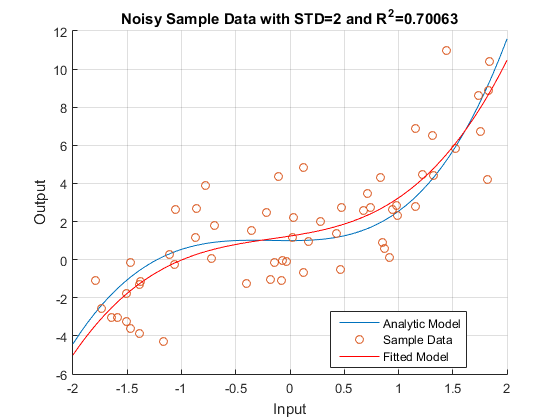
\includegraphics[width=1\linewidth]{plots/case_best.png}
	\end{subfigure}
	\begin{subfigure}{0.49\textwidth} \centering
		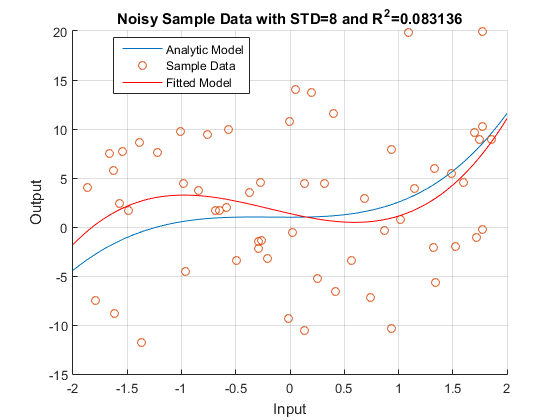
\includegraphics[width=1\linewidth]{plots/case_worst.png}
	\end{subfigure}
	\caption{Noise Study}
	\label{probe 1}
	\end{figure}

We see that if the standard deviation of the noise is half that of
the range of the input, we can get some meaningful results. If the
standard deviation of the noise is double that of the range of the
input, the scatter becomes random. After performing this quick study,
I realized that I can plot the data from the first entry in a similar
fashion and should give an indication of the noise levels in the system.
I also expected to plot a best fit line similar to the plot on the
left with low noise based on what we currently know.

\subsection{Low Q}

The results from the first entry are shown in the subsequent figures.
The first batch of test points that were plagued with data switching
issues and the direct Q measurements performed at the end of the first
entry were excluded. The dynamic pressures for probe 10 and the pressure
readings from all probes are plotted. Note that clusters of points
are visible. The points seem more randomly scatter than having a linear
trend, as evidenced by the negative slope of the curve fit. The plot
below shows the results for the lowest Q setting. The uncertainty
of the measurement is shown in the plus or minus band on the fitted
model. The sorted points are those that were either sampled over a
period of 10 minutes or more or were taken after a warm-up period
of 5 minutes.\begin{figure}[H] \centering
	\begin{subfigure}{0.43\textwidth} \centering
		\includegraphics[width=1\linewidth]{low_q_poly3_10.eps}
	\end{subfigure}
	\begin{subfigure}{0.43\textwidth} \centering
		\includegraphics[width=1\linewidth]{low_q_poly3_all.eps}
	\end{subfigure}
	\begin{subfigure}{0.43\textwidth} \centering
		\includegraphics[width=1\linewidth]{sort_low_q_poly3_10.eps}
	\end{subfigure}
	\begin{subfigure}{0.43\textwidth} \centering
		\includegraphics[width=1\linewidth]{sort_low_q_poly3_all.eps}
	\end{subfigure}
	\caption{Low Q Data with Cubic Fit. From top to bottom: all points and sorted points}
	\end{figure}

\subsection{Medium Q}

The same is shown for the medium Q data. \begin{figure}[H] \centering
	\begin{subfigure}{0.43\textwidth} \centering
		\includegraphics[width=1\linewidth]{med_q_poly3_10.eps}
	\end{subfigure}
	\begin{subfigure}{0.43\textwidth} \centering
		\includegraphics[width=1\linewidth]{med_q_poly3_all.eps}
	\end{subfigure}
	\begin{subfigure}{0.43\textwidth} \centering
		\includegraphics[width=1\linewidth]{sort_med_q_poly3_10.eps}
	\end{subfigure}
	\begin{subfigure}{0.43\textwidth} \centering
		\includegraphics[width=1\linewidth]{sort_med_q_poly3_all.eps}
	\end{subfigure}
	\begin{subfigure}{0.43\textwidth} \centering
		\includegraphics[width=1\linewidth]{med_directq_poly3_10.eps}
	\end{subfigure}
	\begin{subfigure}{0.43\textwidth} \centering
		\includegraphics[width=1\linewidth]{med_directq_poly3_all.eps}
	\end{subfigure}
	\caption{Medium Q Data with Cubic Fit. From top to bottom: all, sorted, and direct reading points} 	\end{figure} 

\subsection{High Q}

\begin{figure}[H] \centering
	\begin{subfigure}{0.43\textwidth} \centering
		\includegraphics[width=1\linewidth]{high_q_poly3_10.eps}
	\end{subfigure}
	\begin{subfigure}{0.43\textwidth} \centering
		\includegraphics[width=1\linewidth]{high_q_poly3_all.eps}
	\end{subfigure}
	\begin{subfigure}{0.43\textwidth} \centering
		\includegraphics[width=1\linewidth]{sort_high_q_poly3_10.eps}
	\end{subfigure}
	\begin{subfigure}{0.43\textwidth} \centering
		\includegraphics[width=1\linewidth]{sort_high_q_poly3_all.eps}
	\end{subfigure}
	\begin{subfigure}{0.43\textwidth} \centering
		\includegraphics[width=1\linewidth]{high_directq_poly3_10.eps}
	\end{subfigure}
	\begin{subfigure}{0.43\textwidth} \centering
		\includegraphics[width=1\linewidth]{high_directq_poly3_all.eps}
	\end{subfigure}
	\caption{High Q Data with Cubic Fit. From top to bottom: all, sorted, and direct reading points}
	\end{figure}

\subsection{Histogram}

Below is a plot of histograms for both the tunnel dynamic pressures
and the probe dynamic pressures where the low, medium, and high Q
cases are shown in each row, respectively, and the tunnel and probe
dynamic pressures are shown left to right. The bin size is equal to
the measurement uncertainty. Two distributions are plotted and their
relative ``goodness of fit'' is shown in the legend, where 1 is
the best fit. I don't know why the metric on the histogram on the
bottom right exceeded 1.\begin{figure}[H] \centering
	\begin{subfigure}{0.43\textwidth} \centering
		\includegraphics[width=1\linewidth]{low_q_hist_tun.eps}
	\end{subfigure}
	\begin{subfigure}{0.43\textwidth} \centering
		\includegraphics[width=1\linewidth]{low_q_hist_probe.eps}
	\end{subfigure}
	\begin{subfigure}{0.43\textwidth} \centering
		\includegraphics[width=1\linewidth]{med_q_hist_tun.eps}
	\end{subfigure}
	\begin{subfigure}{0.43\textwidth} \centering
		\includegraphics[width=1\linewidth]{med_q_hist_probe.eps}
	\end{subfigure}
	\begin{subfigure}{0.43\textwidth} \centering
		\includegraphics[width=1\linewidth]{high_q_hist_tun.eps}
	\end{subfigure}
	\begin{subfigure}{0.43\textwidth} \centering
		\includegraphics[width=1\linewidth]{high_q_hist_probe.eps}
	\end{subfigure}
	\caption{Histogram of Pressure Data}
	\end{figure}

\subsection{Summary}

Tabulated below are the results from the curve-fitting on probe 10.
Fit order refers to whether the fit is linear (1st order) or cubic
(3rd order). R$^{2}$ is a metric of the \textquotedbl{}goodness\textquotedbl{}
of fit. RMSE stands for the root mean square of the error and is a
measure of the standard deviation of the error, or the noise of the
system. NU ratio is something I made up which stands for the noise-to-uncertainty
ratio and is a measure of the system noise to the instrument uncertainty.
\begin{center}
\begin{tabular}{|c|c|c|c|c|}
\hline 
Dynamic Pressure  & Fit Order  & R$^{2}$  & RMSE {[}psf{]}  & NU Ratio \tabularnewline
\hline 
\hline 
Low  & 1  & 0.063  & 0.047  & 0.76 \tabularnewline
\hline 
Low  & 3  & 0.065  & 0.048  & 0.77 \tabularnewline
\hline 
Medium  & 1  & 0.090  & 0.213  & 3.44 \tabularnewline
\hline 
Medium  & 3  & 0.193  & 0.204  & 3.29 \tabularnewline
\hline 
High  & 1  & 0.198  & 0.397  & 6.40 \tabularnewline
\hline 
High  & 3  & 0.270  & 0.384  & 6.19 \tabularnewline
\hline 
\end{tabular}
\par\end{center}

From these results, the low dynamic pressure case exhibits the most
random behavior, especially from the negative linear trends. The medium
but especially the high dynamic pressure case seems to indicate that
the system noise is quite high, higher than the instrument uncertainty.
Cubic fits produce better fits at the medium and high dynamic pressures
suggesting the data is more nonlinear than linear.

\section{Turbulence Intensity}

Given a velocity difference, the associated difference in dynamic
pressure can be calculated using the derivation shown below. If two
measurements are taken, their dynamic pressures can be described as
a function of their respective velocities.

\[
q_{1}=\frac{1}{2}\rho v_{1}^{2}
\]
\[
q_{2}=\frac{1}{2}\rho v_{2}^{2}
\]

If density is assumed constant, the two measurements can be related
as follows:

\[
q_{2}-q_{1}=\frac{1}{2}\rho v_{2}^{2}-\frac{1}{2}\rho v_{1}^{2}
\]
\begin{equation}
\Delta q=\frac{1}{2}\rho(v_{2}^{2}-v_{1}^{2})\label{eq:delq}
\end{equation}

If the difference between the two velocity measurements are small,
they too can be related with a turbulence intensity measurement $T_{i}$,
where turbulence intensity is defined as the ratio between the standard
deviation of the velocity, $\Delta v$, and the mean velocity, $v$
($T_{i}=\Delta v/v$). 
\[
v_{2}-v_{1}=\Delta v=v_{i}\cdot T_{i}
\]
\[
v_{2}=T_{i}\cdot v_{1}+v_{1}
\]
\begin{equation}
v_{2}=(T_{i}+1)\cdot v_{1}\label{eq:vdef}
\end{equation}

\eqref{vdef}and \eqref{delq} can be combined and the subscripts
dropped 
\begin{align}
\Delta q & =\frac{1}{2}\rho(v_{2}^{2}-v_{1}^{2})\nonumber \\
 & =\frac{1}{2}\rho(v_{1}^{2}(T_{i}+1)^{2}-v_{1}^{2})\nonumber \\
 & =\frac{1}{2}\rho(v^{2}(T_{i}^{2}+2T_{i}+1-1))\nonumber \\
\Delta q & =\frac{1}{2}\rho v^{2}(T_{i}^{2}+2T_{i})\label{eq:fin}
\end{align}

\eqref{fin} describes the change in pressure given a turbulence intensity,
$T_{i}$, a mean velocity, $v$, and a density, $\rho$. Given Tina's
measured turbulence intensity without the net installed of 1.5\%,
the turbulence quantities are compared with the measured quantities
at the given velocities. The subscript $t$ denotes turbulence quantities,
the subscript $i$ denotes the calculated ideal value (given incompressible
flow), and the subscript $m$ denotes the measured values from this
experiment. The ideal dynamic pressure, $q_{i}$, is compared with
the measured average dynamic pressure, $\bar{q}_{m}$, by a percent
difference from the ideal. The standard deviation of the dynamic pressure
due to turbulence, $\Delta q_{t}$, is compared with the measured
standard deviation of the experiment (from cubic fit of probe 10),
$\Delta q_{m}$, by a ratio $\Delta q_{t}/\Delta q_{m}$. The values
are tabulated below.
\begin{center}
\begin{tabular}{|c|c|c|c|c|c|c|c|}
\hline 
$v$ {[}ft/s{]}  & $\Delta v_{t}$ {[}ft/s{]}  & $q_{i}$ {[}psf{]}  & $\bar{q}_{m}[psf]$  & Difference $q$  & $\Delta q_{t}$ {[}psf{]}  & $\Delta q_{m}$ {[}psf{]} & Ratio $\Delta q$ \tabularnewline
\hline 
\hline 
140  & 2.10  & 23.30  & 21.76  & -6.64\%  & 0.704  & 0.048  & 0.07 \tabularnewline
\hline 
95  & 1.43  & 10.73  & 10.20  & -4.93\%  & 0.324  & 0.204  & 0.63 \tabularnewline
\hline 
50  & 0.75  & 2.97  & 2.96  & -0.35\%  & 0.090  & 0.384  & 4.27 \tabularnewline
\hline 
\end{tabular}
\par\end{center}

The first thing to note is that the incompressible values for dynamic
pressure match experiment well at the lowest $q$ but get high at
the middle and highest values of $q$. Maybe there are compressible
effects at the wall. The second observation is that the \textquotedbl{}noise\textquotedbl{}
of our system at the lowest $q$ was 4 times greater than that of
the turbulence Tina measured but at middle to high $q$, the \textquotedbl{}noise\textquotedbl{}
of our system is much smaller than the turbulence Tina measured. To
add weight to this analysis, we should consider the uncertainty of
the hot-wire measurement.

\section{Conclusion}

I would like for us to discuss either in person or via e-mail: 
\begin{itemize}
\item any additional testing? We talked briefly over Mike's luncheon that
if we saw anything \textquotedbl{}bad\textquotedbl{} we'd have to
re-do even more but is this considered \textquotedbl{}bad\textquotedbl{}?
We were very consistent in how we acquired the data (go up to condition,
immediately take data). Do we want to re-run this matrix once the
reference line is in place? 
\item any additional plots? I didn't show the 90 deg/270 deg and clocking
effects so I can include that later. 
\item does this change anything about below-lip entry? 
\item data hand-off. Currently I'm using MATLAB to call and process the
data - are you OK with me showing you how to use my code if you or
someone else in the future wants to look at the data? Documentation
will go along with that.
\end{itemize}
furthermore:
\begin{itemize}
\item Do we continue using the rake? Do we need to complement with another
tool, like smoke viz or PIV? 
\item Do we measure below the lip? Do we need any repeat runs? What's the
priority, repeat runs or below the lip? 
\item Are there implications for the SARL characterization effort? 
\item Would CFD be useful and where/how? 
\end{itemize}
\begin{thebibliography}{1}
\bibitem{key-1}
\end{thebibliography}
\pagebreak{}

\section{Appendix: Run Log}

Below is the log of the test (make the font smaller on this run log)

\section{Appendix: Log}
\end{document}
